% THIS IS SIGPROC-SP.TEX - VERSION 3.1
% WORKS WITH V3.2SP OF ACM_PROC_ARTICLE-SP.CLS
% APRIL 2009
%
% Questions regarding SIGS should be sent to
% Adrienne Griscti ---> griscti@acm.org
%
% Questions/suggestions regarding the guidelines, .tex and .cls files, etc. to
% Gerald Murray ---> murray@hq.acm.org
%
% For tracking purposes - this is V3.1SP - APRIL 2009
%
% Copied from https://github.com/heathermiller/papers-documents/tree/master/rem2013

\documentclass{support/acm_proc_article-sp}
\usepackage{listings}
\usepackage{url}
\usepackage{support/bcprules}
\usepackage{support/prooftree}
\usepackage{support/math}
\usepackage{multicol}
\usepackage{caption}
\usepackage{subcaption}
\usepackage[normalem]{ulem}
\usepackage{color}
\usepackage{graphicx}
\usepackage{hyperref}

\renewcommand{\thesubsection}{\thesection.\alph{subsection}}

\definecolor{blue}{rgb}{0,0,0.5}
\definecolor{red}{rgb}{0.6,0,0}
\definecolor{green}{rgb}{0,0.5,0}
\definecolor{grey}{rgb}{0.2,0.2,0.2}

\lstdefinelanguage{Python}{
keywords={typeof, null, catch, switch, in, int, str, float, self},
keywordstyle=\color{blue}\bfseries,
ndkeywords={boolean, throw, import},
ndkeywords={return, class, if ,elif, endif, while, do, else, True, False , catch, def},
ndkeywordstyle=\color{blue}\bfseries,
identifierstyle=\color{red},
sensitive=false,
comment=[l]{\#},
morecomment=[s]{/*}{*/},
commentstyle=\color{green}\ttfamily,
stringstyle=\color{green}\ttfamily,
}

\lstset{language=Python}

% comments and notes
\newcommand{\comment}[1]{}
\newcommand{\note}[1]{{\bf $\clubsuit$ #1 $\spadesuit$}}
\newcommand{\ifreport}[1]{#1}
%\newcommand{\ifreport}[1]{}

\newcommand{\todo}{{\bf \colorbox{red}{\color{white}TODO:}}}
\newcommand{\ie}{{\em i.e.,~}}
\newcommand{\eg}{{\em e.g.,~}}
\newcommand{\term}[1]{\mbox{\texttt{#1}}}
\newcommand{\itl}[1]{\mbox{\textit{#1}}}

% commas and semicolons
\newcommand{\comma}{,\,}
\newcommand{\commadots}{\comma \ldots \comma}
\newcommand{\semi}{;\mbox{;};}
\newcommand{\semidots}{\semi \ldots \semi}

% spacing
\newcommand{\gap}{\quad\quad}
\newcommand{\biggap}{\quad\quad\quad}
\newcommand{\nextline}{\\ \\}
\newcommand{\htabwidth}{0.5cm}
\newcommand{\tabwidth}{1cm}
\newcommand{\htab}{\hspace{\htabwidth}}
\newcommand{\tab}{\hspace{\tabwidth}}
\newcommand{\linesep}{\ \hrulefill \ \smallskip}

\newcommand{\sectionline}{%
\nointerlineskip \vspace{\baselineskip}%
\hspace{\fill}\rule{0.5\linewidth}{.7pt}\hspace{\fill}%
\par\nointerlineskip \vspace{\baselineskip}
}

% figures
\newcommand{\figurebox}[1]
{\fbox{\begin{minipage}{\textwidth}
           #1 \medskip
\end{minipage}}}
\newcommand{\twofig}[3]
{\begin{figure*}[t]
     #3\ \hrulefill\
        \caption{\label{#1}#2}
\end{figure*}}
\newcommand{\boxfig}[3]
{\begin{figure*}
     \figurebox{#3\caption{\label{#1}#2}}
\end{figure*}}
\newcommand{\figref}[1]
{Figure~\ref{#1}}

% arrays
\newcommand{\ba}{\begin{array}}
\newcommand{\ea}{\end{array}}
\newcommand{\bda}{\[\ba}
\newcommand{\eda}{\ea\]}
\newcommand{\ei}{\end{array}}
\newcommand{\bcases}{\left\{\begin{array}{ll}}
\newcommand{\ecases}{\end{array}\right.}

\pagenumbering{arabic}
\begin{document}

    \title{Hot Topics in Machine Learning (HWS17) \\ Assignment 2: Naive Bayes}

    \numberofauthors{1}
    \author{
    \alignauthor
    Steffen Schmitz\\
    \affaddr{University of Mannheim}\\
    \affaddr{stefschm@mail.uni-mannheim.de}
    }

    \maketitle

    %%%%%%%%%%%%%%%%%%%%%%%%%%%%%%%%%%%%%%%%%%%%%%%%%%%%
    %%
    %% 1) TRAINING
    %%
    %%%%%%%%%%%%%%%%%%%%%%%%%%%%%%%%%%%%%%%%%%%%%%%%%%%%

    \section{Training}
    \label{sec:training}

    \textbf{Task.} Provide a function that trains a Naive Bayes classifier for categorical data using a symmetric Dirichlet
    prior and MAP parameter estimates.

    We want to use a Naive Bayes classifier to assign probabilities to each possible class-label given a new, previously
    unseen datapoint.
    Given Bayes' rule we say that
    \begin{equation}
        P(Y | X) = \frac{P(Y)P(X | Y)}{P(X)} \propto P(Y)P(X | Y)
        \label{eq:bayes}
    \end{equation}
    where $P(Y | X)$ is the probability or our posterior belief that $Y = y$ for a specific datapoint $x$.

    Following Murphy \cite[p.65]{Murphy:2012:MLP:2380985} we can use the proportionality of Equation \ref{eq:bayes} to predict
    the class-label of a feature vector $x$.
    Therefor, we need to compute the class-conditional densities $P(X | Y)$ for each class $y$ and the prior class
    probability $P(Y)$.

    To compute the prior we can maximize the Multinomial distribution which would lead to a Maximum Likelihood Estimate (MLE)
    that is equal to the relative frequencies of each category in the training data.
    This can result in a zero-count problem, when a category does not appear in the test data.
    Using a symmetric Dirichlet prior we obtain the Maximum a Posteriori estimation (MAP) that is computed as
    \begin{equation}
        \hat{\theta}_{MAP} = \frac{n_1 + \alpha - 1 \mbox{  } n_2 + \alpha - 1 \mbox{ ... } n_K + \alpha - 1}{n + K \cdot \alpha - K}
    \end{equation}
    with $\alpha \in \mathbb{R}^+$ and $\alpha = 1$ being equal to the MLE.

    The Python implementation is shown in Figure \ref{fig:prior}.
    \begin{figure}[htbp]
        \centering
        \lstset{numbers=none,xleftmargin=0em}
        \lstinputlisting{listings/prior.py}
        \caption{Prior class probability.}
        \label{fig:prior}
    \end{figure}

    For the class-conditional densities we compute the number of occurrences of each feature for every class and apply
    the same formula as above.
    \begin{figure}[htbp]
        \centering
        \lstset{numbers=none,xleftmargin=0em}
        \lstinputlisting{listings/likelihood.py}
        \caption{Class-conditional densities.}
        \label{fig:cc-densities}
    \end{figure}

    We combine the implementations in Figure \ref{fig:prior} and Figure \ref{fig:cc-densities} to define the nb\_train
    method that returns both results in logarithmic form.

    %%%%%%%%%%%%%%%%%%%%%%%%%%%%%%%%%%%%%%%%%%%%%%%%%%%%
    %%
    %% 2) PREDICTION
    %%
    %%%%%%%%%%%%%%%%%%%%%%%%%%%%%%%%%%%%%%%%%%%%%%%%%%%%

    \section{Predition}
    \label{sec:prediction}

    \textbf{Task.} Provide a function that takes your model and a set of examples, and outputs the most likely label for
    each example as well as the log probability (confidence) of that label.

    In this exercise we will implement a function that takes in a model that we trained with the function from Section \ref{sec:training}
    and use it to compute our belief that a new feature vector $x$ belongs to a specific class.

    We know from Equation \ref{eq:bayes} that we need to compute the product of the prior class probability and the class-conditional
    densities to obtain the probability that a feature vector $x$ belongs into class $y$.
    If we do this computation in logarithm-space we obtain the log-likelihood and can use sums instead of products.
    This leads to Equation \ref{eq:log-likelihood} \cite[p.83]{Murphy:2012:MLP:2380985}.
    \begin{equation}
        \ell(\mathbf{X}, \mathbf{y} | \mathbf{\theta}) = \sum_{c = 1}^C n_c \log \pi_c + \sum_{j = 1}^D \sum_{c = 1}^C \sum_{i: y_i = c} \log [\theta_{jc}] x_{ij}
        \label{eq:log-likelihood}
    \end{equation}
    We compute the log-likelihood for each possible class for each feature vector $x$ and use the maximum result as
    our prediction.

    %%%%%%%%%%%%%%%%%%%%%%%%%%%%%%%%%%%%%%%%%%%%%%%%%%%%
    %%
    %% 3) EXPERIMENTS ON MNIST DIGITS DATA
    %%
    %%%%%%%%%%%%%%%%%%%%%%%%%%%%%%%%%%%%%%%%%%%%%%%%%%%%

    \section{Experiments on MNIST digits data}

    \subsection{Accuracy}

    \textbf{Task.} Train your model with $\alpha = 2$ on the MNIST training dataset, then predict the labels of the MNIST test
    data using your model.
    What is accuracy of your model?

    If we create a model and make predictions as explained in Section \ref{sec:prediction} we obtain an accuracy of
    83.6\% on the MNIST-dataset\footnote{\href{http://yann.lecun.com/exdb/mnist/}{http://yann.lecun.com/exdb/mnist/}}.
    This is equal to the accuracy that we get by applying the Multinomial Naive Bayes algorithm from the scikit-learn
    Python package\footnote{\href{http://scikit-learn.org/stable/modules/generated/sklearn.naive_bayes.MultinomialNB.html}{http://scikit-learn.og/MultionmialNB.html}}.
    The scikit-learn Bernoulli Naive Bayes program performs a little better and has an accuracy of 84.1\% on the testset.

    Given that the result is the same as the scikit-learn implementation we can conclude that our Naive Bayes implementation
    is reasonable.

    Nevertheless it should be possible to get much better prediction results.
    The TensorFlow documentation states that a result of 92\% accuracy is fairly bad for a simple neural network and
    that they can get results of around 99.2\% with a Multilayer Convolutional Neural
    Network\footnote{\href{https://www.tensorflow.org/get_started/mnist/pros\#build_a_multilayer_convolutional_network}{https://tensorflow.org/multilayer\_cnn}}.

    \subsection{Error discussion}

    \textbf{Task.} Plot some test digits for each predicted class label.
    Can you spot errors?
    Then plot some misclassified test digits for each predicted class label.
    Finally, compute the confusion matrix.
    Discuss the errors the model makes.

    First, we look at the predicted classifications of a sample of images and later analyse the confusion matrix.
    Figure \ref{fig:predicted-images} shows some images from the testset grouped by the predicted class label.
    This Figure contains images with a wrong label and images with a correct label.
    Due to the accuracy of 83,6\% we would expect 125 of the 150 images to have the correct label (Actual: 24 misclassifications).
    \begin{figure}[!htbp]
        \centering
        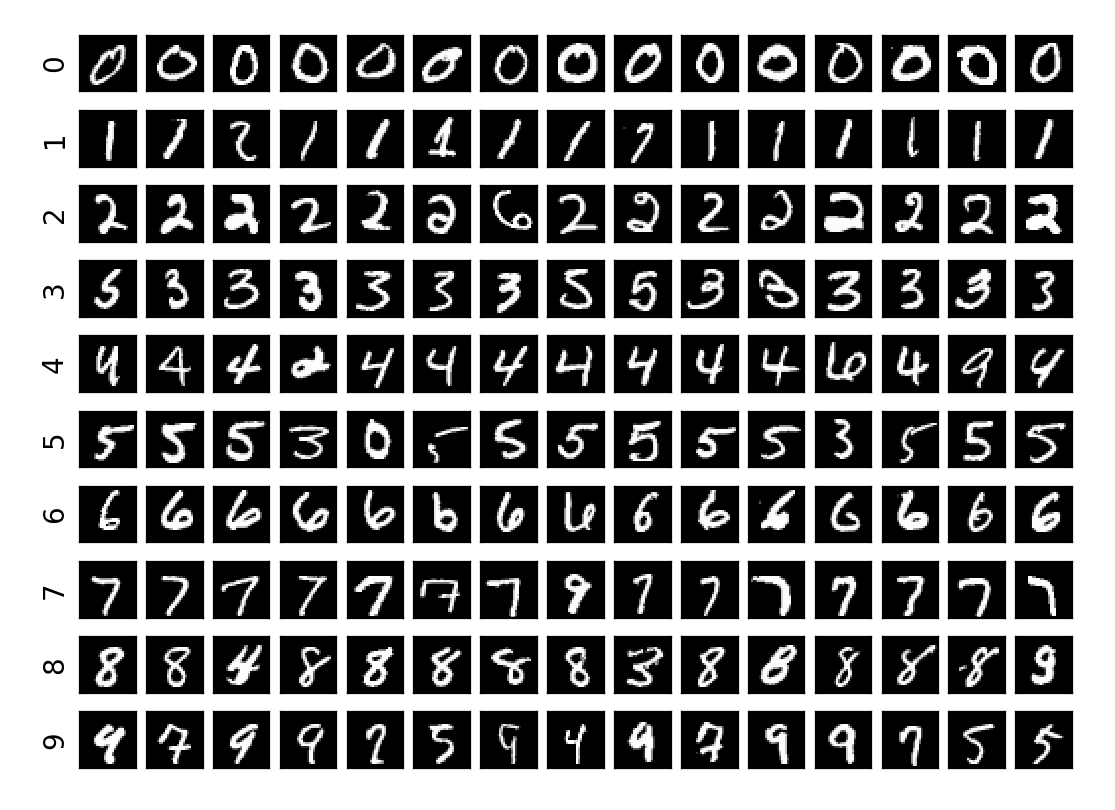
\includegraphics[width=8cm]{images/predicted-images.png}
        \caption{Digits grouped by predicted label}
        \label{fig:predicted-images}
    \end{figure}

    We can see that most of the misclassifications share some characteristics with the surrounding data and for some
    images it is even for a human hard to classify the number correctly.
    Compare for example the images in the first column for images labeled as "4" and "9".
    Although they look very similar they are classified differently and the label is ambiguous.

    Now we will look at the classification report (Figure \ref{fig:classification-report}) and the confusion matrix
    (Figure \ref{fig:confusion-matrix}) to quantify our notion of the results.
    \begin{figure}[!htbp]
        \centering
        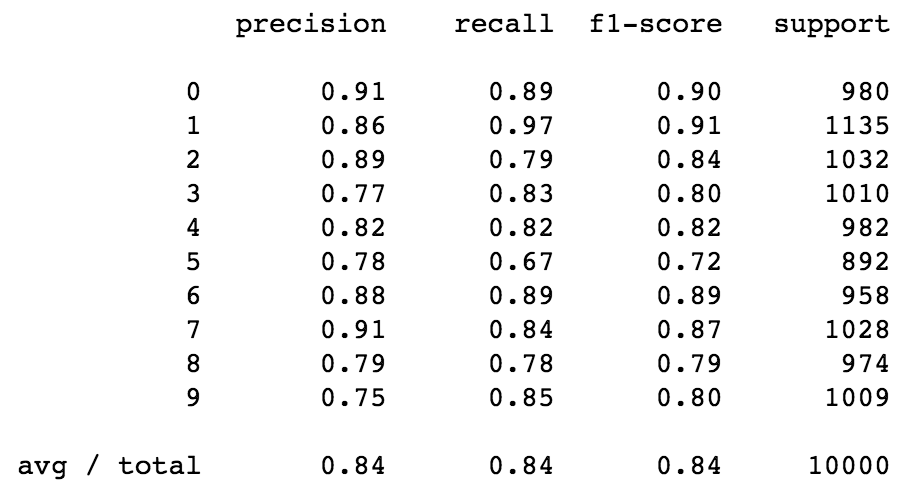
\includegraphics[width=8cm]{images/classification-report.png}
        \caption{Classification Report}
        \label{fig:classification-report}
    \end{figure}
    We can see in the Classification Report that the labels 0, 1 and 7 have the highest F1-Score (around 0.9) and are
    therefor predicted most accurately.
    This could be explained by the shape of 1 and 7 that is very different from the rather round shapes that all other
    elements have in common.
    A possible explanation of the high F1-Score of 0 might be, that there aren't many ways to write a 0, but for example
    multiple ways to write a 4.

    The worst F1-Score has the number 5 with a score of 0.72.
    This is caused by the very low recall of 0.67.
    The recall is defined as the ratio between True Positives (TP) and True Positives and False Negatives (FN) \cite{evaluation}.
    \begin{equation}
        Recall = \frac{TP}{TP + FN}
    \end{equation}
    This means that it is more unlikely, compared to all other classes, that the classifier will detect the true class
    label of an input feature vector that should be labeled as a 5.

    \begin{figure}[!htbp]
        \centering
        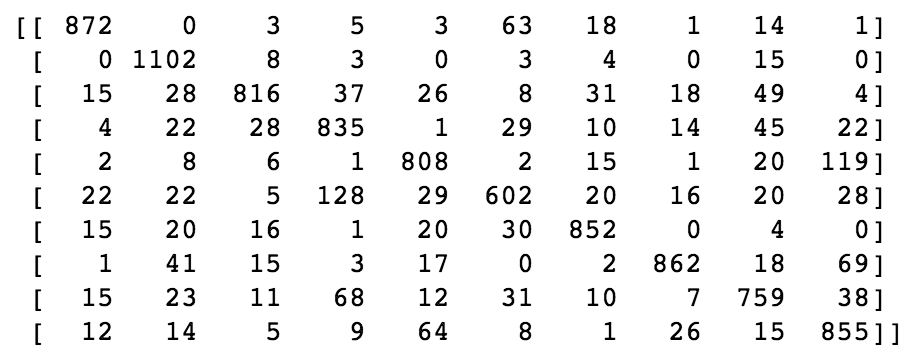
\includegraphics[width=8cm]{images/confusion-matrix.png}
        \caption{Confusion Matrix}
        \label{fig:confusion-matrix}
    \end{figure}
    We can see from the confusion matrix that there are 63 cases where a 0 is interpreted as a 5 and 128 cases where
    a 3 is predicted to be a 5.
    Especially the confusion between a 3 and a 5 may be explained through the various ways to write the 5.

    All in all we can conclude that our classifier is easily confused by similarities between numbers that
    are caused by the specific handwriting style.

    %%%%%%%%%%%%%%%%%%%%%%%%%%%%%%%%%%%%%%%%%%%%%%%%%%%%
    %%
    %% 4) MODEL SELECTION
    %%
    %%%%%%%%%%%%%%%%%%%%%%%%%%%%%%%%%%%%%%%%%%%%%%%%%%%%

    \section{Model selection}
    \label{sec:model-selection}

    \textbf{Task.} Use cross-validation to find a suitable value of the hyperparameter $\alpha$ (of the symmetric Dirichlet prior).
    Also plot the accuracy (as estimated via cross-validation) as a function of $\alpha$.
    Discuss.

    For cross-validation we split our labeled training data into $K$ random folds that have a similar size.
    We use $K - 1$ of them to train our model and the remaining one to calculate the accuracy of our trained model.
    This procedure has the advantage that we can tune our hyperparamater without touching our test data.
    If we use our optimized model on the test data afterwards we obtain an unbiased result of how well our model
    works on real or previously unseen data.

    \begin{figure}[htbp]
        \centering
        \lstset{numbers=none,xleftmargin=0em}
        \lstinputlisting{listings/k-fold.py}
        \caption{K-Fold Model Selection.}
        \label{fig:k-fold}
    \end{figure}
    Figure \ref{fig:k-fold} shows how we approach this with $K = 5$.
    For each fold we receive a labeled training set and a labeled test set that we can use to calculate the accuracy.
    Then we create a model and run a prediction on the test set and compare it with the true values.
    In the end we save the accuracy in a list with the corresponding alpha and afterwards we can just look up the
    maximum accuracy and use the alpha at this index.

    In the notebook we try $\alpha \in [2, 6]$ and get 82,8\% accuracy as the best result with $\alpha = 2$.
    The results for all $\alpha$ are shown in Figure \ref{fig:k-fold-accuracy}.
    \begin{figure}[!htbp]
        \centering
        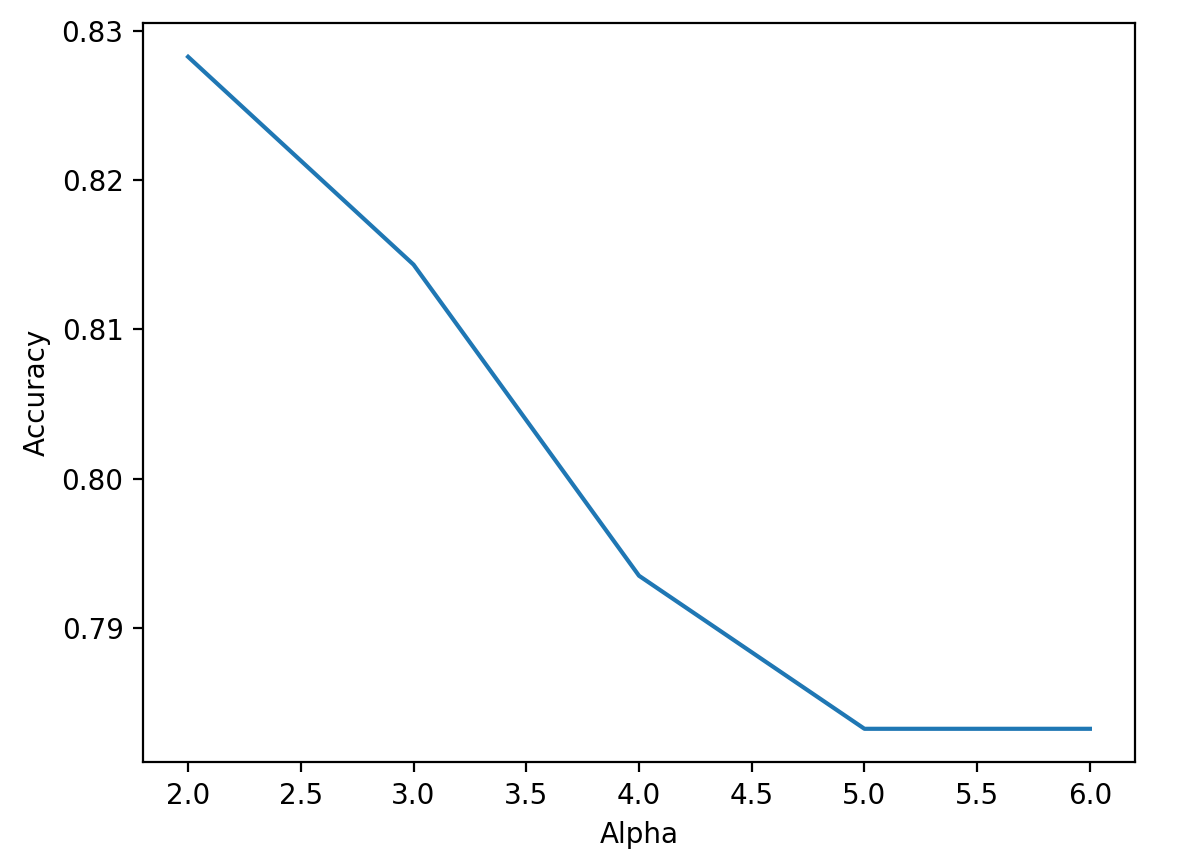
\includegraphics[width=8cm]{images/k-fold.png}
        \caption{$\alpha$ - Accuracy}
        \label{fig:k-fold-accuracy}
    \end{figure}

    %%%%%%%%%%%%%%%%%%%%%%%%%%%%%%%%%%%%%%%%%%%%%%%%%%%%
    %%
    %% 5) GENERATING DATA
    %%
    %%%%%%%%%%%%%%%%%%%%%%%%%%%%%%%%%%%%%%%%%%%%%%%%%%%%

    \section{Generating data}

    \subsection{Generation}

    \textbf{Task.} Implement a function that generates digits for a set of provided list of class labels.

    We use the log-likelihoods that are stored in our model to create vectors, given a class label.
    Here we can use \lstinline{np.random.choice(range(K), p=prob)} to generate a random sample
    with the probabilities associated with each entry of the first
    parameter\footnote{\href{https://docs.scipy.org/doc/numpy-1.13.0/reference/generated/numpy.random.choice.html}{https://docs.scipy.org/numpy.random.choice.html}}.
    \begin{figure}[htbp]
        \centering
        \lstset{numbers=none,xleftmargin=0em}
        \lstinputlisting{listings/generation.py}
        \caption{Generate data.}
        \label{fig:generation}
    \end{figure}
    We do this generation for each element in the list of class labels and for each feature.

    \subsection{Interpretation}

    \textbf{Task.} Generate some digits of each class for your trained model and plot.
    Interpret the result.
    Repeat data generation for different models by varying the hyperparameter $\alpha$.
    How does $\alpha$ influence the results?
    Discuss.

    The result of the digit generation is displayed in Figure \ref{fig:generated-digits}.
    We can see that the resulting images look "cloudy", but most of them are still identifiable as the class label that
    they should represent.
    \begin{figure}[!htbp]
        \centering
        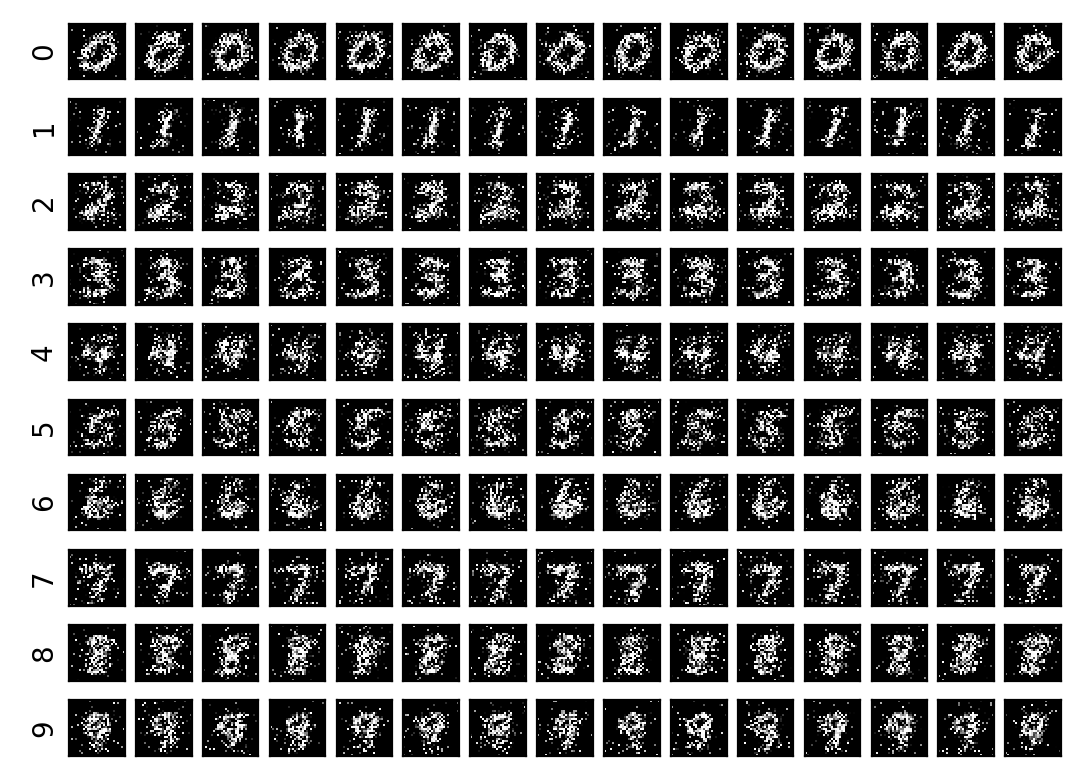
\includegraphics[width=8cm]{images/generated-digits.png}
        \caption{Some generated digits for each class}
        \label{fig:generated-digits}
    \end{figure}
    The "cloudyness" can be explained through the randomization that calculates the color or each pixel individually
    without looking left or right.
    This means that creating a line, where neighbouring pixels have a similar color, is not taken into account during the
    image generation.

    If we repeat this process for increasing values of alpha, the accuracy of our generated models decreases.
    While the white dots were clustered in the center for $\alpha = 2$ they appear also around the edges of the image
    for increasing alphas.

    Interpreting $\alpha$ as a pseudo count of prior observations we can conclude that a large $\alpha$ leads to
    a larger prior belief for each possible pixel in our image.
    This is caused by the usage of the symmetric Dirichlet prior.
    Given more training data we would expect the number of points that are close to the edges to go down and to have
    them clustered around the middle and to resemble to class label for closely.

    This is also supported by the observation from Section \ref{sec:model-selection} that larger $\alpha$s reduce the
    accuracy of our predictions.

    %%%%%%%%%%%%%%%%%%%%%%%%%%%%%%%%%%%%%%%%%%%%%%%%%%%%
    %%
    %% 6) PREPROCESSING FEATURES AND GAUSSIAN NB
    %%
    %%%%%%%%%%%%%%%%%%%%%%%%%%%%%%%%%%%%%%%%%%%%%%%%%%%%

    \section{Preprocessing features and Gaussian Naive Bayes}

    \textbf{Task.} Try to find a better Naive Bayes classifier.
    E.g., you may try to preprocess features or to use a continuous Naive Bayes classifier.
    Can you improve on the Naive Bayes classifiers obtained in the previous tasks?
    What is the best accuracy you can get?

    \subsection{Preprocessing}

    One way to preprocess the features is to binarize them.
    In our input set we deal with features in a range from 0 to 255 representing different shades of grey.
    If we binarize them we may reduce the complexity and think of each pixel in the input image as being either
    black or white.

    We use the sklearn.preprocessing.Binarizer to make each feature either 0 or
    1\footnote{\href{http://scikit-learn.org/stable/modules/generated/sklearn.preprocessing.Binarizer.html}{http://scikit-learn.org/Binarizer.html}}.

    This results in an accuracy of 84.2\% which is around 0.6\% better than the accuracy on unpreprocessed data.

    \subsection{Gaussian Naive Bayes}

    The Gaussian Naive Bayes implementation in the sklearn.naive\_bayes package assumes that all features have a
    Gaussian distribution and estimates the mean and variance using maximum
    likelihood\footnote{\href{http://scikit-learn.org/stable/modules/naive_bayes.html\#gaussian-naive-bayes}{http://scikit-learn.org/naive\_bayes.html}}.

    If we use it on the unprocessed input data like in Figure \ref{fig:gaussian} we obtain an accuracy of 55.6\% which
    is worse than our accuracy of 83.6\% for the unnormalized categorical model.
    \begin{figure}[htbp]
        \centering
        \lstset{numbers=none,xleftmargin=0em}
        \lstinputlisting{listings/gaussian.py}
        \caption{Applying Gaussian Naive Bayes.}
        \label{fig:gaussian}
    \end{figure}

    The best result we obtained is 84.2\% accuracy with a binarized input and a categorical Naive Bayes implementation.

    %%%%%%%%%%%%%%%%%%%%%%%%%%%%%%%%%%%%%%%%%%%%%%%%%%%%
    %%
    %% BIBLIOGRAPHY
    %%
    %%%%%%%%%%%%%%%%%%%%%%%%%%%%%%%%%%%%%%%%%%%%%%%%%%%%

    \bibliographystyle{abbrv}
    \bibliography{support/bib}

\end{document}
